\documentclass{report}
\usepackage{graphicx} % Required for inserting images
\usepackage{todonotes}
\usepackage{amsmath}
\usepackage{amsfonts}
\usepackage{hyperref}
\title{Application of Right for the Right Reasons}

\newcommand{\itodo}[1]{\todo[inline]{#1}}
\newcommand{\vtodo}[1]{\todo[inline,color=purple!50!white]{#1}}

\date{January 2025}
\author{Vladyslav Zlochevskyi}

\begin{document}

\maketitle

\begin{abstract}
 Deep learning techniques, while advancing the state of the art in numerous domains, remain opaque,
 posing significant challenges for critical applications where trust and interpretability are strong requirement.
 This paper extends the research in Explanatory Interactive Learning (XIL) focusing on ``Right for the Right Reasons''
 methodology.
 RRR introduces a novel loss function to align model explanations with human-intuitive reasoning, building trust and reliability.
 We present experiments utilizing the MNIST dataset, where models are trained under conventional and RRR paradigms.
 We demonstrate that RRR enhances interpretability by mitigating confounding factors and aligning decision-making with
 intuitive patterns, as validated by Grad-CAM and Guided Grad-CAM explainers.
\end{abstract}

\tableofcontents

\chapter{Introduction}
\label{ch:introduction}

In recent years, deep learning techniques have advanced significantly, bringing increased complexity and a lack of transparency.
A relatively new concept, Generative AI, has achieved results that would have been unimaginable a decade ago.
These include breakthroughs in areas such as Natural Language Processing (NLP) and the creation of artwork that rivals human expertise.

However, the models underlying these achievements are highly non-interpretable.
While they are effective and produce correct outputs in most cases, we often lack a comprehensive understanding of
how they function and why they make specific decisions.
This opacity raises critical questions, especially when considering the application of such models in critical infrastructure,
where incorrect decisions could lead to catastrophic outcomes.
At present, these models are not deployed in such contexts due to the absence of human trust in their decision-making processes.

This paper aims to advance research in \emph{Explanatory Interactive Learning} (XIL),
a concept designed to foster trust by ensuring that models are trained to be ``right for the right reasons''.

\chapter{Theory}
\label{ch:theory}

\section{Supervised classification}
\label{sec:sup-class}
\subsection{Neural Network}
\label{subsec:neural-network}
A model in Machine Learning refers to a mathematical representation of a process that has been trained on data.
One of the most critical properties of a model is its ability to encapsulate the patterns inherent in the data.
A neural network (NN) is a specific type of Machine Learning model designed to mimic
the operational patterns of neurons in the animal brain.

A neural network consists of layers.
The basic structure includes an input layer, an output layer, and multiple hidden layers situated between the two.
Each layer comprises nodes that are interconnected with nodes from adjacent layers.
Each node receives \emph{signals} from connected nodes, processes them, and transmits a new signal to other connected nodes.
This \emph{signal} is a numerical value derived by applying an \emph{activation function} to
the \emph{weighted signals from the previous layer}.
Signals are weighted using weights, which are assigned to the relationships from which the signals originate.
\begin{itemize}
    \item Data sent to the input layer is referred to as ``inputs'' or ``Xs.''
    \item Data produced by the output layer is referred to as ``outputs'' or ``predictions.''
    \item Data representing the expected results of processed inputs is referred to as ``targets,'' ``labels,'' or ``ys.''
\end{itemize}

The relationship between inputs and predictions can be expressed as $\hat{y} = f_{\theta}(X)$,
where $\theta$ represents the vector of learnable parameters.

Supervised Learning is a Machine Learning technique that utilizes \emph{labels} to train a model
capable of predicting correct outputs.
Other techniques, such as unsupervised learning, generally do not rely on \emph{labels}.

To evaluate the performance of a model, \emph{loss} or \emph{cost functions} are defined.
These functions measure the deviation of the model's predictions from the ``ground truth''.
Minimizing the \emph{loss} calculated by the cost function can improve the model's performance.

To minimize the loss, Machine Learning employs optimization techniques called \emph{optimizers}.
One of the simplest optimization methods is \emph{Stochastic Gradient Descent} (SGD).
During SGD execution, weights are updated as follows (as described in~\cite{Li_2018}):
\begin{equation}
 \label{eq:sgd}
 \boldsymbol{\theta}^{[new]} = \boldsymbol{\theta}^{[old]} - \mu \boldsymbol{P} \boldsymbol{\hat{g}}(\boldsymbol{\theta}^{[old]}) \text{,}
 \end{equation}
where $\boldsymbol{\theta}$ denotes learnable parameters, $\mu$ represents the learning rate,
$\boldsymbol{\hat{g}}(\boldsymbol{\theta}^{[old]})$ are the gradients of the learnable parameters,
and $\boldsymbol{P}$ is a matrix known as the ``preconditioner''.
In most training sessions, $\boldsymbol{P}$ is set to $\boldsymbol{I}$, the \emph{identity matrix},
in which case the optimizer is referred to as ``plain'' SGD\@.

In this paper, we utilize the \emph{Adaptive Moment Estimation} optimizer, commonly known as \emph{ADAM}.
This optimizer is a special case of preconditioned SGD and is defined as follows (as described in~\cite{kingma2017adammethodstochasticoptimization}):
\begin{align}
 m_t = \beta_1 m_{t - 1} + (1 - \beta_1) g_t \\
 v_t = \beta_2 v_{t - 1} + (1 - \beta_2) g_t^2 \\
 \hat{m_t} = \frac{m_t}{1 - \beta_1^t} \\
 \hat{v_t} = \frac{v_t}{1 - \beta_2^t} \\
 \theta_t = \theta_{t - 1} - \mu \frac{\hat{m_t}}{(\sqrt {\hat{v_t}} + \epsilon)} \text{,}
\end{align}
where $t$ is a discrete timestep, $g_t = \nabla_\theta f_t (\theta_{t - 1})$, $\beta_1$ and $\beta_2$ are hyperparameters.
Notably, $\beta_i^t$ represents $\beta_i$ raised to the power of $t$, and $g_t^2$ indicates the elementwise square $g_t \cdot g_t$.

As optimizers require the computation of gradients for every weight in the model, most deep learning frameworks
provide tools for \emph{Automatic Differentiation} (AD), as discussed in~\cite{JMLR:v18:17-468}
and implemented in the \emph{PyTorch} framework~\cite{paszke2017automatic}.

\subsection{Cross-entropy loss function}
\label{subsec:cross-entropy-loss}
The cross-entropy loss function is a specialized loss function commonly used for supervised classification tasks.
It is defined as:
\[L = -\frac{1}{N} \sum_{i=1}^{N} \sum_{j=1}^{C} y_{ij} \log(\hat{y}_{ij}) \text{,}\]
where $N$ represents the number of examples, and $C$ denotes the number of classes.

\emph{Cross-entropy loss} function is derived by taking negative loglikelihood of \emph{Bernoulli distribution}(\ref{eq:bernoulli-likelihood}).

\begin{equation}
 \label{eq:bernoulli-likelihood}
 P(y | \hat{y}) = \hat{y}^y (1 - \hat{y})^{1-y}
\end{equation}

\subsection{Convolutional Neural Network}
\label{subsec:convolutional-neural-network}
Convolutional Neural Network (aka CNN) is a type of Neural Network, that is well-suited for image recognition.
It is usually made up of such multiple layers as:
\begin{itemize}
 \item \textbf{Convolutional layers}: layers, which apply convolutional operations to input, using \emph{filters} (aka kernels).
 These kind of operations help to detect complex features such as edges, textures and other patterns.
 \item \textbf{Pooling layers}: layers, which reduce spatial dimensions of the input.
 These operations decrease computational complexity - speed up processing.
 \item \textbf{Activation Function layers}: non-linear activation functions,
 which add non-linearity to the model and help model to learn more complex relationships in the data.
 The most common such layer is \emph{Rectified Linear Unit} (ReLU)
 \item \textbf{Fully connected layers (aka Dense layers)}: this layer connect every neuron to every neuron of the next layer.
\end{itemize}

\section{Explanations}
\label{sec:explanations}

\subsection{Grad-CAM}
\label{subsec:gradcam}
\emph{Gradient-weighted Class Activation Mapping (Grad-CAM)} is an explanation technique introduced in the work
by~\cite[Grad-CAM: Visual Explanations from Deep Networks via Gradient-based Localization]{Selvaraju_2019}.
It generates \emph{visual explanations} for the decisions made by the vast majority of convolutional neural network (CNN)-based models.
Grad-CAM utilizes the gradients of the target concept that flow into the final convolutional layer to produce a localization map.
This map highlights regions of the input image that contributed significantly to the model's prediction.

According to~\cite{Selvaraju_2019}, the \emph{class-discriminative localization map},
denoted as $L_{\text{Grad-CAM}}^c \in \mathbb{R}^{u \times v}$ for any class $c$, is computed as follows:
\begin{samepage}
    \[\alpha_k^c = \overbrace{\frac{1}{Z} \sum_i^u \sum_j^v}^{\text{global average pooling}}
    \underbrace{\frac{\partial y^c}{\partial A_{ij}^k}}_{\text{gradients via backprop}}\]

    \[L_{Grad-CAM}^c = ReLU(\underbrace{\sum_k \alpha_k^c A^k}_{\text{linear combination}}) \quad \text{,}\]
\end{samepage}
where $y^c$ represents the score for class $c$, $A^k$ denotes the $k$-th feature map activations of the convolutional layer,
and $Z = u \cdot v$ is the normalization factor.

\subsection{Guided Grad-CAM}
\label{subsec:guided-gradcam}

\emph{Guided Grad-CAM}~\cite{Selvaraju_2019} is an enhanced version of \emph{Grad-CAM} (Subsection~\ref{subsec:gradcam}),
designed to highlight fine-grained details in contrast to \emph{Grad-CAM}, which primarily identifies ``relevant'' regions.

Before delving into the computation of \emph{Guided Grad-CAM},
it is essential to discuss one of its foundational components: \emph{Guided Backpropagation}.
This pixel-space gradient visualization technique was proposed by \emph{Springenberg}~\cite{springenberg2014striving}.

The process begins with a forward pass of the input data up to the convolutional layer of interest, as illustrated in Figure~\ref{fig:guided_backprop_forward}.
Following this, the image is ``reconstructed'' through a backward pass, as depicted in Figure~\ref{fig:guided_backprop_backward},
and is mathematically summarized in Equation~\ref{eq:guided-backprop}.

\begin{equation}
 R_i^l = (f_i^l > 0) \cdot (R_i^{l+1} > 0) \cdot R_i^{l+1} \text{,}
 \label{eq:guided-backprop}
\end{equation}

where $R_i^{l+1} = \frac{\partial \text{out}}{\partial f_i^{l+1}}$.

\begin{figure}
 \centering
 \includegraphics[width=0.75\textwidth]{imgs/guided_backpropagation_1}
 \caption{Forward pass of the image~\cite{springenberg2014striving}}
 \label{fig:guided_backprop_forward}
\end{figure}

\begin{figure}
 \centering
 \includegraphics[width=0.75\textwidth]{imgs/guided_backpropagation_2}
 \caption{Backward pass of the output to ``reconstruct'' the image~\cite{springenberg2014striving}}
 \label{fig:guided_backprop_backward}
\end{figure}

\emph{Guided Grad-CAM} combines the strengths of both \emph{Guided Backpropagation} and \emph{Grad-CAM}.
It is computed as the element-wise multiplication of the ``reconstructed image'' obtained from \emph{Guided Backpropagation}
and the attention map generated by \emph{Grad-CAM}, which is upsampled to the resolution of the input image using
\emph{bilinear interpolation}, as described in~\cite{Selvaraju_2019}.

\section{Right for the right reasons}
\label{sec:rrr-theory}
\emph{Right for the Right Reasons} is a loss function for a differentiable model proposed by~\cite{ross2017right}
and modified by~\cite{schramowski2020making}.
The \emph{Right for the Right Reasons} loss (hereafter referred to as \emph{RRR loss}) is defined as follows:

\begin{samepage}
 \begin{equation}
  \label{eq:rrr-right-answers}
  L(\theta, X, y, A) = \sum_{n=1}^{N} \sum_{k=1}^{K} -c_k y_{nk} \log (\hat{y}_{nk}) \quad \text{(Right answers)}
  \end{equation}

 \begin{equation}
  \label{eq:rrr-right-reasons}
  + \lambda_1 \sum_{n=1}^{N} \sum_{d=1}^{D} \left( A_{nd} \frac{\delta}{\delta h_{nd}} \sum_{k=1}^{K} c_k \log (\hat{y}_{nk}) \right)^2 \quad \text{(Right reasons)}
 \end{equation}

 \begin{equation}
  \label{eq:rrr-l2-reg}
  + \lambda_2 \sum_{i} \theta_i^2 \quad \text{(Weight regularization)}
  \end{equation}
\end{samepage}
where $\theta$ is a vector of weights, $X$ represents the inputs, $y$ denotes the labels, $A$ refers to binary masks,
$c$ is a class weight, $\hat{y}$ represents the predictions, and $h$ is the feature map of the convolutional layer,
typically the final one.
$N$ denotes the number of examples, $K$ is the number of classes produced by the model,
and $D$ is the number of features in the feature map.

The \emph{RRR loss}'s ``right answers'' component, shown in Equation~(\ref{eq:rrr-right-answers}),
is derived from the \emph{Cross-entropy loss} function (Subsection~\ref{subsec:cross-entropy-loss}) and is modified to incorporate class weights.
The ``weight regularization'' component, given in Equation~(\ref{eq:rrr-l2-reg}),
employs standard L2 regularization to mitigate overfitting in the model.

The novel contribution of this loss function lies in the ``right reasons'' component, outlined in Equation~(\ref{eq:rrr-right-reasons}).
This term penalizes large gradients of the convolutional layer in regions indicated by binary masks.
The $\lambda$ parameters are used to balance the contributions of the different regularization terms.
As described in~\cite{ross2017right}, the regularization parameter $\lambda_{1}$ should be chosen such
that the ``right answers'' and ``right reasons'' terms are of comparable magnitudes.

We propose a modification to the ``right reasons'' component of this loss function,
specifically in Equation~(\ref{eq:rrr-right-reasons}).
Our modification introduces an additional summation across all convolutional layers of interest,
as presented in Equation~(\ref{eq:rrr-modified}):
\begin{align}
 L(\theta, X, y, A) = \sum_{n=1}^{N} \sum_{k=1}^{K} -c_k y_{nk} \log (\hat{y}_{nk}) \\
 + \lambda_1 \frac{1}{L}\sum_{l=1}^{L} \sum_{n=1}^{N} \sum_{d=1}^{D} \left( A_{nd} \frac{\delta}{\delta h_{nd}^{l}} \sum_{k=1}^{K} c_k \log (\hat{y}_{nk}) \right)^2 \label{eq:rrr-modified} \\
 + \lambda_2 \sum_{i} \theta_i^2
\end{align}

It is also important to note that in implementations of the \emph{RRR loss},
binary masks are generated with the size of the original input,
rather than the size of the feature maps from the convolutional layers of interest.
During the computation of the loss,
each binary mask is then downscaled to the size of the respective convolutional layer using bilinear interpolation.

\chapter{Experiments}
\label{ch:experiments}
Before conducting a more complex experiment,
we decided to begin with a simpler one that would illustrate the core aspects of the proposed methodology
and help identify the tools and techniques requiring further attention.

In summary, the steps we aim to undertake are as follows:
\begin{enumerate}
\item Select a specific dataset for a classification task;
\item Train a model using the \emph{common approach};
\item Experiment with various explainers and choose the one that provides explanations aligned with our requirements;
\item Identify a scenario in which the model trained with the common approach fails to perform adequately;
\item Retrain the model using the novel approach, i.e., \emph{RRR Loss} (Subsection~\ref{sec:rrr-theory});
\item Demonstrate that the newly trained model eliminates confounding factors as part of the classification explanation.
\end{enumerate}

\section{MNIST}
\label{sec:08-mnist}

Before delving into the MNIST experiment, we first describe the training parameters that apply to most of the trainings discussed in this subsection.
Any deviations from these parameters will be noted explicitly.

\begin{itemize}
 \item \textbf{Model architecture}: The architecture of our model consists of the following sequence of layers,
 as illustrated in Figure~\ref{fig:08_cnn_architecture}:
 \begin{enumerate}
    \item Convolutional layer with kernel size $3 \times 3$, stride = 1, padding = 1
    \item ReLU activation layer
    \item MaxPool layer with kernel size $2 \times 2$, stride = 2
    \item Convolutional layer with kernel size $3 \times 3$, stride = 1, padding = 1
    \item ReLU activation layer
    \item MaxPool layer with kernel size $2 \times 2$, stride = 2
    \item Flattening layer from $32 \times 7 \times 7$ to $1568$
    \item Fully connected layer from $1568$ to $128$
    \item ReLU activation layer
    \item Fully connected layer from $128$ to $2$
    \item Softmax layer
 \end{enumerate}
 \item \textbf{Optimizer}: ADAM($\beta_1 = 0.9$, $\beta_2 = 0.999$, learning rate = 0.001)
 \item \textbf{Loss function}: Cross Entropy Loss or \emph{RRR Loss}.
 \item \textbf{Other training details}: Batch size = 64, number of epochs = 2, training data size = 11,773, test data size = 1,954.
\end{itemize}

\begin{figure}
 \centering
 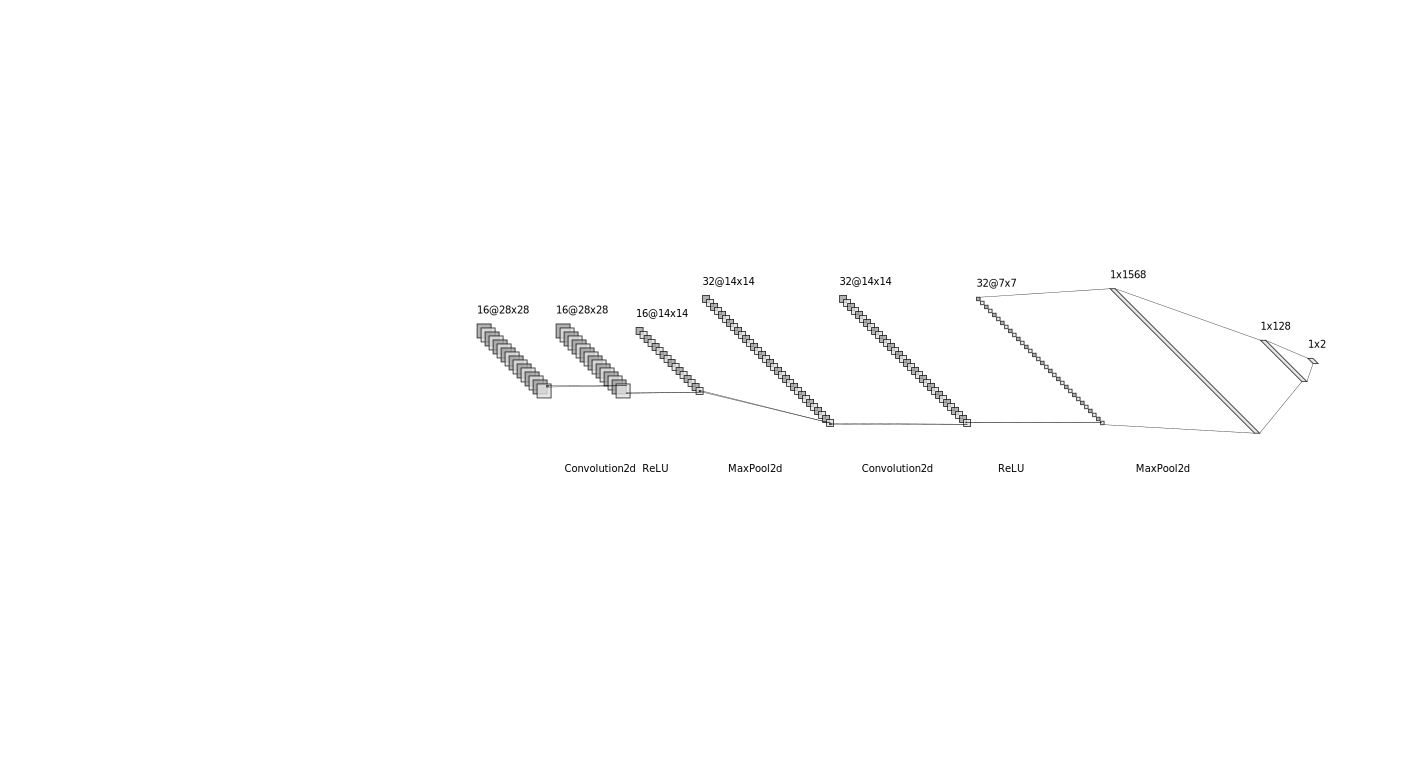
\includegraphics[width=\textwidth]{imgs/08_mnist_cnn}
 \caption{Architecture of the CNN used in MNIST experiment.}
 \label{fig:08_cnn_architecture}
\end{figure}

Thus, we utilize the standard \emph{MNIST} dataset~\cite{deng2012mnist} and restrict it to contain only zeros and eights.
This choice is made because an intuitive explanation for distinguishing between these two classes should focus
on the middle part of the image, where eights display a ``cross'' as illustrated in Figure~\ref{fig:08_diff}.
This is precisely the feature we expect the explainer to annotate as the \emph{right reason} for the classification.

\begin{figure}
 \centering
 \includegraphics{imgs/zero_eight_diff}
 \caption{Intuitive difference between 0 and 8.}
 \label{fig:08_diff}
\end{figure}

\subsection{Comparison of explainers}
\label{subsec:comparison-of-explainers}

In this section, we describe our choice of explainer.
The primary criterion was to select a `model-agnostic' explainer.
Consequently, we began with the Grad-CAM series of explainers and ultimately selected the basic Grad-CAM method (Section~\ref{subsec:gradcam}).

The model performs well, and we observe that the attention map generated by Grad-CAM (Figure~\ref{fig:gradcam_exp})
provides a clear explanation of the regions of the instances that contribute to the prediction.
However, it does not offer sufficient insight into the precise differences between the instances,
rendering it less informative in this regard.

\begin{figure}
 \centering
 \includegraphics[width=0.5\textwidth]{imgs/exp_2_5_gradcam}
 \caption{Grad-CAM attention map.}
 \label{fig:gradcam_exp}
\end{figure}

Therefore, we decided to employ Guided Grad-CAM (Section~\ref{subsec:guided-gradcam}),
as it provides a more detailed explanation than Grad-CAM.
As shown in Figure~\ref{fig:guided_gradcam_exp}, we have somewhat achieved our objective:
the model distinguishes between zeros and eights based on the intuition we proposed earlier in Figure~\ref{fig:08_diff}.

\begin{figure}
 \centering
 \includegraphics[width=0.5\textwidth]{imgs/exp_2_5_guided_gradcam}
 \caption{Guided Grad-CAM attention map.}
 \label{fig:guided_gradcam_exp}
\end{figure}

\subsection{Undertrained model's explanations}
\label{subsec:undertrained-model's-explanations}
We also aimed to investigate the explanations provided by the model when it is undertrained.
To achieve this, we trained the model on a subset of 200 samples for 3 epochs.
The accuracy of the model reached $93\%$.
Upon applying Grad-CAM (Subsection~\ref{subsec:gradcam}),
we were surprised to observe (Figure~\ref{fig:gradcam_on_poor_model}) that the model learned
to differentiate between eights and zeros based on the background, rather than the silhouette of the object.
We hypothesize that such a model would perform poorly in real-world deployment, especially if the background is filled with noise.

\begin{figure}
 \centering
 \includegraphics[width=0.75\textwidth]{imgs/gradcam_on_poor_adam}
 \caption{Grad-CAM applied on the undertrained model}
 \label{fig:gradcam_on_poor_model}
\end{figure}

\subsection{Artificial dataset}
\label{subsec:artificial-dataset}

In the previous subsection, we demonstrated that our trained model performed well,
and its explanations of the classification tasks appeared to be satisfactory.
However, what occurs when we create a dataset that may contain an additional \emph{not necessarily helpful} pattern?
This situation is effectively described
in~\cite[Overfitting occurs when the machine-learning model captures the regularities of data it has been trained on arbitrarily closely,
 but its predictions’ accuracy does not transfer well to unseen test data, that is, it fits the noise]{thomas2024modelling}.

To explore this, we decided to add a dot to every sample of eight in our dataset,
as illustrated in Figure~\ref{fig:dotted_ds}, in order to simulate a dataset gathered from a \emph{limited environment}.
\begin{figure}
 \centering
 \includegraphics[width=0.5\textwidth]{imgs/zero_eight_dot}
 \caption{A pair of zero and "dotted" eight.}
 \label{fig:dotted_ds}
\end{figure}

We trained the model on this dataset and applied Guided Grad-CAM.
Although the accuracy remains comparable to that of the model trained on the unmodified dataset,
the explanation for classifying eights predominantly originates from the added dot (Figure~\ref{fig:guided-gradcam-dotted}).
Furthermore, when evaluating the model on the unmodified dataset, the accuracy may decrease to $60\%$, as shown in Table~\ref{tab:avg-accuracy-rrr}.

\begin{table}
 \label{tab:avg-accuracy-rrr}
 \centering
 \caption{Table showing average accuracy of the model trained with RRR loss function throughout 3 executions.}
\begin{tabular}{|l||c|c|}
 \hline
 Average accuracy with RRR loss & Train dataset & Test dataset \\
 \hline \hline
 $\lambda_1=0;\lambda_2=0$ & $100\%$ & $65,8\%$ \\
 \hline
 $\lambda_1=2;\lambda_2=0$ & $99,8\%$ & $97,9\%$ \\
 \hline
\end{tabular}
\end{table}

\begin{figure}
 \centering
 \includegraphics[width=0.5\textwidth]{imgs/exp_4_dotted_8_gradcam}
 \caption{Guided Grad-CAM on dotted dataset.}
 \label{fig:guided-gradcam-dotted}
\end{figure}

\subsection{RRR}
\label{subsec:rrr}
At this stage of our experiment, we retrain the model using the \emph{same} hyperparameters,
\emph{same} model architecture, and \emph{same} optimizer.
However, we replace the previously used Cross-entropy loss function with the \emph{right for the right reasons} loss function
(Section~\ref{sec:rrr-theory}). Regarding the binary masks required by the RRR method, we define them as follows:
1) set the values to 1 in the region of the dot; 2) set the values to 0 elsewhere.

\begin{figure}
 \centering
 \includegraphics[width=0.5\textwidth]{imgs/exp_4_dotted_guided_gradcam_rrr}
 \caption{Guided Grad-CAM on dotted dataset. Model trained with RRR.}
 \label{fig:guided-gradcam-dotted-rrr}
\end{figure}

As shown in Figure~\ref{fig:guided-gradcam-dotted-rrr}, our model has learned to reject the dot.
Furthermore, it has successfully learned to differentiate between zeros and eights based on the intuition we suggested in Figure~\ref{fig:08_diff}.

\chapter{Plans and improvements}
\label{ch:plans-improvements}
This chapter outlines our plans and ideas for further developing different aspects of this bachelor thesis:

\begin{itemize}
    \item \textbf{Codebase}: The cam overlay does not currently function with Guided Grad-CAM.
    We plan to address and resolve this issue.
    \item \textbf{Data Scope}: We aim to extend the application of the described techniques to other types of data,
    such as EKG data from patients.
    \item \textbf{Scenario}: We intend to explore a scenario where creating binary masks is costly.
    Specifically, we plan to investigate a situation where the number of available binary masks is very low,
    and the model would learn without them.
    For the most uncertain samples, it would query for the binary mask.
    For example, in some domains, an expert in the relevant field is required to create the binary masks, which can be time-consuming and expensive.
    \item \textbf{Sensitive Study}: We plan to investigate our ``08 MNIST'' experiment in greater detail by addressing the following question:
    ``What if there are $n$ samples of eights that do not have the dot?
    How many such samples ($n$) would be needed to achieve accuracy (and the `right reason') comparable to the RRR method?''
    \item \textbf{Art of Binary Masks}: Different approaches can be applied when creating binary masks for the RRR method or other techniques.
    For example, in~\cite{ross2017right}, it is noted that ``At the other extreme, when A is a matrix of all 1s, it encourages the model to have small gradients
    with respect to its inputs; this can improve generalization on its own''~\cite{ross2017right}.
\end{itemize}
\itodo{Trust study. I guess, the main goal of XIL, except for correcting the model to be RRR, is building trust. Im thinking, that at some point we would need to do a survey}\vtodo{Survey of what? Poll between users?}\itodo{I guess yeah, I think that if we'll get some more time after the main experiments, it would be nice to have a survey, which would compare user's trust to the model trained commonly and the model trained with XIL. Well if it is needed...}

\chapter{Conclusion}
\label{ch:conclusion}

In this work, we conducted a smaller-scale experiment, ``08 MNIST'', to explore the tools necessary for researching Explanatory Interactive Learning (XIL).
We set clear expectations for this experiment and believe we have successfully met them.
However, as outlined in Chapter~\ref{ch:plans-improvements}, there are several scenarios that warrant further investigation.

\emph{Explainability Methods}.
We experimented with \emph{Grad-CAM} and \emph{Guided Grad-CAM} for generating explanations.
These methods performed well in the context of our specific experiment.
However, as discussed earlier, the choice of explanation method is highly dependent on both the model and the goals of the experiment.
Therefore, in future work, we may need to explore alternative explanation techniques, as we do not yet fully
understand the full scope of advantages provided by the methodology.

\emph{Right for the Right Reasons (RRR)}.
The \emph{Right for the Right Reasons} loss function produced good and expected results in our experiment.
Although we did not delve into the so-called ``art of creating binary masks'',
we followed a straightforward approach for constructing them:
we manually created ``dots'' in the artificial dataset, which made it relatively easy to generate corresponding binary masks.
However, one important question remains:
What if we had chosen to penalize gradients in the static regions ``where dots may appear''?
How would this influence the final model performance?
During our experiment, we encountered different approaches to creating binary masks,
and it is evident that this ``art'' should not be underestimated.

\emph{Further Research}.
Most of our future research directions have been outlined in Chapter~\ref{ch:plans-improvements}.
In particular, we plan to explore the effects of different binary mask generation strategies,
investigate more complex datasets, and extend the methodology to other domains.

\bibliographystyle{plain}
\bibliography{bib}
\end{document}
